%%%%%%%%%%%%%%%%%%%%%%%%%%%%%%%%%%%%%%%%%%%%%%%%%%%%%%%%%%%%%%%%%%%%%%%%%%
%
% 	Template for seminar reports
%
%%%%%%%%%%%%%%%%%%%%%%%%%%%%%%%%%%%%%%%%%%%%%%%%%%%%%%%%%%%%%%%%%%%%%%%%%%

%%%%%%%%%%%%%%%%%%%%%%%%%%%%%%%%%%%%%%%%%%%%%%%%%%%%%%%%%%%%%%%%%%%%%%%%%%
% 	Include layout and macros
%%%%%%%%%%%%%%%%%%%%%%%%%%%%%%%%%%%%%%%%%%%%%%%%%%%%%%%%%%%%%%%%%%%%%%%%%%


%% This LaTeX template is based on the following example file included in the ieeetran
%% package:
%% bare_conf.tex 
%% V1.2
%% 2002/11/18
%% by Michael Shell
%% mshell@ece.gatech.edu
%% (requires IEEEtran.cls version 1.6b or later) with an IEEE conference paper.


% Note that the a4paper option is mainly intended so that authors in
% countries using A4 can easily print to A4 and see how their papers will
% look in print. Authors are encouraged to use U.S. letter paper when 
% submitting to IEEE. Use the testflow package mentioned above to verify
% correct handling of both paper sizes by the author's LaTeX system.
%
% Also note that the "draftcls" or "draftclsnofoot", not "draft", option
% should be used if it is desired that the figures are to be displayed in
% draft mode.
%
% This paper can be formatted using the peerreviewca
% (instead of conference) mode.
\documentclass[conference, a4paper]{IEEEtran-modified}
% If the IEEEtran.cls has not been installed into the LaTeX system files, 
% manually specify the path to it:
% \documentclass[conference]{../sty/IEEEtran} 

\IEEEoverridecommandlockouts

% some very useful LaTeX packages include:

\usepackage{cite}       % Written by Donald Arseneau
                        % V1.6 and later of IEEEtran pre-defines the format
                        % of the cite.sty package \cite{} output to follow
                        % that of IEEE. Loading the cite package will
                        % result in citation numbers being automatically
                        % sorted and properly "ranged". i.e.,
                        % [1], [9], [2], [7], [5], [6]
                        % (without using cite.sty)
                        % will become:
                        % [1], [2], [5]--[7], [9] (using cite.sty)
                        % cite.sty's \cite will automatically add leading
                        % space, if needed. Use cite.sty's noadjust option
                        % (cite.sty V3.8 and later) if you want to turn this
                        % off. cite.sty is already installed on most LaTeX
                        % systems. The latest version can be obtained at:
                        % http://www.ctan.org/tex-archive/macros/latex/contrib/supported/cite/

%\usepackage{graphicx}  % Written by David Carlisle and Sebastian Rahtz
                        % Required if you want graphics, photos, etc.
                        % graphicx.sty is already installed on most LaTeX
                        % systems. The latest version and documentation can
                        % be obtained at:
                        % http://www.ctan.org/tex-archive/macros/latex/required/graphics/
                        % Another good source of documentation is "Using
                        % Imported Graphics in LaTeX2e" by Keith Reckdahl
                        % which can be found as esplatex.ps and epslatex.pdf
                        % at: http://www.ctan.org/tex-archive/info/
% NOTE: for dual use with latex and pdflatex, instead load graphicx like:
\ifx\pdfoutput\undefined
	\usepackage{graphicx}
\else
	\usepackage[pdftex]{graphicx}
\fi

% However, be warned that pdflatex will require graphics to be in PDF
% (not EPS) format and will preclude the use of PostScript based LaTeX
% packages such as psfrag.sty and pstricks.sty. IEEE conferences typically
% allow PDF graphics (and hence pdfLaTeX). However, IEEE journals do not
% (yet) allow image formats other than EPS or TIFF. Therefore, authors of
% journal papers should use traditional LaTeX with EPS graphics.
%
% The path(s) to the graphics files can also be declared: e.g.,
% \graphicspath{{../eps/}{../ps/}}
% if the graphics files are not located in the same directory as the
% .tex file. This can be done in each branch of the conditional above
% (after graphicx is loaded) to handle the EPS and PDF cases separately.
% In this way, full path information will not have to be specified in
% each \includegraphics command.
%
% Note that, when switching from latex to pdflatex and vice-versa, the new
% compiler will have to be run twice to clear some warnings.
\graphicspath{{figures/}}


%\usepackage{psfrag}    % Written by Craig Barratt, Michael C. Grant,
                        % and David Carlisle
                        % This package allows you to substitute LaTeX
                        % commands for text in imported EPS graphic files.
                        % In this way, LaTeX symbols can be placed into
                        % graphics that have been generated by other
                        % applications. You must use latex->dvips->ps2pdf
                        % workflow (not direct pdf output from pdflatex) if
                        % you wish to use this capability because it works
                        % via some PostScript tricks. Alternatively, the
                        % graphics could be processed as separate files via
                        % psfrag and dvips, then converted to PDF for
                        % inclusion in the main file which uses pdflatex.
                        % Docs are in "The PSfrag System" by Michael C. Grant
                        % and David Carlisle. There is also some information 
                        % about using psfrag in "Using Imported Graphics in
                        % LaTeX2e" by Keith Reckdahl which documents the
                        % graphicx package (see above). The psfrag package
                        % and documentation can be obtained at:
                        % http://www.ctan.org/tex-archive/macros/latex/contrib/supported/psfrag/

%\usepackage{subfigure} % Written by Steven Douglas Cochran
                        % This package makes it easy to put subfigures
                        % in your figures. i.e., "figure 1a and 1b"
                        % Docs are in "Using Imported Graphics in LaTeX2e"
                        % by Keith Reckdahl which also documents the graphicx
                        % package (see above). subfigure.sty is already
                        % installed on most LaTeX systems. The latest version
                        % and documentation can be obtained at:
                        % http://www.ctan.org/tex-archive/macros/latex/contrib/supported/subfigure/

%\usepackage{url}       % Written by Donald Arseneau
                        % Provides better support for handling and breaking
                        % URLs. url.sty is already installed on most LaTeX
                        % systems. The latest version can be obtained at:
                        % http://www.ctan.org/tex-archive/macros/latex/contrib/other/misc/
                        % Read the url.sty source comments for usage information.

%\usepackage{stfloats}  % Written by Sigitas Tolusis
                        % Gives LaTeX2e the ability to do double column
                        % floats at the bottom of the page as well as the top.
                        % (e.g., "\begin{figure*}[!b]" is not normally
                        % possible in LaTeX2e). This is an invasive package
                        % which rewrites many portions of the LaTeX2e output
                        % routines. It may not work with other packages that
                        % modify the LaTeX2e output routine and/or with other
                        % versions of LaTeX. The latest version and
                        % documentation can be obtained at:
                        % http://www.ctan.org/tex-archive/macros/latex/contrib/supported/sttools/
                        % Documentation is contained in the stfloats.sty
                        % comments as well as in the presfull.pdf file.
                        % Do not use the stfloats baselinefloat ability as
                        % IEEE does not allow \baselineskip to stretch.
                        % Authors submitting work to the IEEE should note
                        % that IEEE rarely uses double column equations and
                        % that authors should try to avoid such use.
                        % Do not be tempted to use the cuted.sty or
                        % midfloat.sty package (by the same author) as IEEE
                        % does not format its papers in such ways.

\usepackage{amsmath}    % From the American Mathematical Society
                        % A popular package that provides many helpful commands
                        % for dealing with mathematics. Note that the AMSmath
                        % package sets \interdisplaylinepenalty to 10000 thus
                        % preventing page breaks from occurring within multiline
                        % equations. Use:
\interdisplaylinepenalty=2500
                        % after loading amsmath to restore such page breaks
                        % as IEEEtran.cls normally does. amsmath.sty is already
                        % installed on most LaTeX systems. The latest version
                        % and documentation can be obtained at:
                        % http://www.ctan.org/tex-archive/macros/latex/required/amslatex/math/



% Other popular packages for formatting tables and equations include:

%\usepackage{array}
% Frank Mittelbach's and David Carlisle's array.sty which improves the
% LaTeX2e array and tabular environments to provide better appearances and
% additional user controls. array.sty is already installed on most systems.
% The latest version and documentation can be obtained at:
% http://www.ctan.org/tex-archive/macros/latex/required/tools/

% Mark Wooding's extremely powerful MDW tools, especially mdwmath.sty and
% mdwtab.sty which are used to format equations and tables, respectively.
% The MDWtools set is already installed on most LaTeX systems. The lastest
% version and documentation is available at:
% http://www.ctan.org/tex-archive/macros/latex/contrib/supported/mdwtools/


% V1.6 of IEEEtran contains the IEEEeqnarray family of commands that can
% be used to generate multiline equations as well as matrices, tables, etc.


% Also of notable interest:

% Scott Pakin's eqparbox package for creating (automatically sized) equal
% width boxes. Available:
% http://www.ctan.org/tex-archive/macros/latex/contrib/supported/eqparbox/



% Notes on hyperref:
% IEEEtran.cls attempts to be compliant with the hyperref package, written
% by Heiko Oberdiek and Sebastian Rahtz, which provides hyperlinks within
% a document as well as an index for PDF files (produced via pdflatex).
% However, it is a tad difficult to properly interface LaTeX classes and
% packages with this (necessarily) complex and invasive package. It is
% recommended that hyperref not be used for work that is to be submitted
% to the IEEE. Users who wish to use hyperref *must* ensure that their
% hyperref version is 6.72u or later *and* IEEEtran.cls is version 1.6b 
% or later. The latest version of hyperref can be obtained at:
%
% http://www.ctan.org/tex-archive/macros/latex/contrib/supported/hyperref/
%
% Also, be aware that cite.sty (as of version 3.9, 11/2001) and hyperref.sty
% (as of version 6.72t, 2002/07/25) do not work optimally together.
% To mediate the differences between these two packages, IEEEtran.cls, as
% of v1.6b, predefines a command that fools hyperref into thinking that
% the natbib package is being used - causing it not to modify the existing
% citation commands, and allowing cite.sty to operate as normal. However,
% as a result, citation numbers will not be hyperlinked. Another side effect
% of this approach is that the natbib.sty package will not properly load
% under IEEEtran.cls. However, current versions of natbib are not capable
% of compressing and sorting citation numbers in IEEE's style - so this
% should not be an issue. If, for some strange reason, the user wants to
% load natbib.sty under IEEEtran.cls, the following code must be placed
% before natbib.sty can be loaded:
%
\makeatletter
\let\NAT@parse\undefined
\makeatother
%
% Hyperref should be loaded differently depending on whether pdflatex
% or traditional latex is being used:
%
\ifx\pdfoutput\undefined
\usepackage[hypertex]{hyperref}
\else
\usepackage[pdftex,hypertexnames=false]{hyperref}
\fi
%
% Pdflatex produces superior hyperref results and is the recommended
% compiler for such use.



% *** Do not adjust lengths that control margins, column widths, etc. ***
% *** Do not use packages that alter fonts (such as pslatex).         ***
% There should be no need to do such things with IEEEtran.cls V1.6 and later.

%
%%%%%%%%%%%%%%%%%%%%%%%%%%%%%%%%%%%%%%%%%%%%%%%%%%%%%%%%%%%%%%%%%%%%%%%%%%
% 	Anpassung an deutsche Texte
%%%%%%%%%%%%%%%%%%%%%%%%%%%%%%%%%%%%%%%%%%%%%%%%%%%%%%%%%%%%%%%%%%%%%%%%%%

\usepackage{ngerman}
\usepackage[latin1]{inputenc}   % f�r Umlaute 

\renewcommand{\abstractname}{Kurzfassung}      % statt Zusammenfassung, wie es ngerman definiert
\renewcommand{\keywordname}{Schl�sselworte}
%\renewcommand{\figurename}{Abb.}




%%%%%%%%%%%%%%%%%%%%%%%%%%%%%%%%%%%%%%%%%%%%%%%%%%%%%%%%%%%%%%%%%%%%%%%%%%
% 	Page numbering (not on first page)
%%%%%%%%%%%%%%%%%%%%%%%%%%%%%%%%%%%%%%%%%%%%%%%%%%%%%%%%%%%%%%%%%%%%%%%%%%
\pagestyle{plain}

%%%%%%%%%%%%%%%%%%%%%%%%%%%%%%%%%%%%%%%%%%%%%%%%%%%%%%%%%%%%%%%%%%%%%%%%%%
% 	Correct bad hyphenation here
%%%%%%%%%%%%%%%%%%%%%%%%%%%%%%%%%%%%%%%%%%%%%%%%%%%%%%%%%%%%%%%%%%%%%%%%%%

\hyphenation{}

%%%%%%%%%%%%%%%%%%%%%%%%%%%%%%%%%%%%%%%%%%%%%%%%%%%%%%%%%%%%%%%%%%%%%%%%%%
% 	Begin of the document
%%%%%%%%%%%%%%%%%%%%%%%%%%%%%%%%%%%%%%%%%%%%%%%%%%%%%%%%%%%%%%%%%%%%%%%%%%

\begin{document}

%%%%%%%%%%%%%%%%%%%%%%%%%%%%%%%%%%%%%%%%%%%%%%%%%%%%%%%%%%%%%%%%%%%%%%%%%%
% 	Paper title
%%%%%%%%%%%%%%%%%%%%%%%%%%%%%%%%%%%%%%%%%%%%%%%%%%%%%%%%%%%%%%%%%%%%%%%%%%

\title{Title of your Work}

%%%%%%%%%%%%%%%%%%%%%%%%%%%%%%%%%%%%%%%%%%%%%%%%%%%%%%%%%%%%%%%%%%%%%%%%%%
% 	Author names and affiliations 
%		-	multiple columns for up to three different affilitations are separated 
%			by \and
%		- for over three affiliations, refer to ieeetran howto
%%%%%%%%%%%%%%%%%%%%%%%%%%%%%%%%%%%%%%%%%%%%%%%%%%%%%%%%%%%%%%%%%%%%%%%%%%

\author{
\authorblockN{FirstName A. SecondName}
\authorblockA{Department of Informatics\\ Technical University of Munich\\
Email: name@in.tum.de} 
%\and
%\authorblockN{}
%\authorblockA{}
}

%%%%%%%%%%%%%%%%%%%%%%%%%%%%%%%%%%%%%%%%%%%%%%%%%%%%%%%%%%%%%%%%%%%%%%%%%%
% 	Special paper note (appears between title and authors) 
%%%%%%%%%%%%%%%%%%%%%%%%%%%%%%%%%%%%%%%%%%%%%%%%%%%%%%%%%%%%%%%%%%%%%%%%%%

\specialpapernotice{Title of the Seminar}

%%%%%%%%%%%%%%%%%%%%%%%%%%%%%%%%%%%%%%%%%%%%%%%%%%%%%%%%%%%%%%%%%%%%%%%%%%
% 	Make title area 
%%%%%%%%%%%%%%%%%%%%%%%%%%%%%%%%%%%%%%%%%%%%%%%%%%%%%%%%%%%%%%%%%%%%%%%%%%

\maketitle

%%%%%%%%%%%%%%%%%%%%%%%%%%%%%%%%%%%%%%%%%%%%%%%%%%%%%%%%%%%%%%%%%%%%%%%%%%
% 	For page number on first page
%%%%%%%%%%%%%%%%%%%%%%%%%%%%%%%%%%%%%%%%%%%%%%%%%%%%%%%%%%%%%%%%%%%%%%%%%%

%\thispagestyle{plain}

%%%%%%%%%%%%%%%%%%%%%%%%%%%%%%%%%%%%%%%%%%%%%%%%%%%%%%%%%%%%%%%%%%%%%%%%%%
% 	Abstract 
%%%%%%%%%%%%%%%%%%%%%%%%%%%%%%%%%%%%%%%%%%%%%%%%%%%%%%%%%%%%%%%%%%%%%%%%%%


\begin{abstract}
Surveillance capitalism has raised significant ethical concerns regarding the collection and utilization of personal data by tech giants like Google.
This paper explores these ethical implications through various ethical frameworks, including deontological ethics, consequentialism, and hedonism.
The analysis reveals critical issues related to privacy, autonomy, and fairness, and proposes potential solutions to mitigate these concerns.
By examining case studies of Google's practices, including data breaches and unauthorized data collection, the paper highlights the need for stricter regulations and ethical data practices to protect user rights in the digital age.
Ensuring transparency, informed consent, and robust data protection measures are essential for balancing the benefits of data-driven innovation with respect for individual rights.
\end{abstract}


%%%%%%%%%%%%%%%%%%%%%%%%%%%%%%%%%%%%%%%%%%%%%%%%%%%%%%%%%%%%%%%%%%%%%%%%%%
% 	Keywords 
%%%%%%%%%%%%%%%%%%%%%%%%%%%%%%%%%%%%%%%%%%%%%%%%%%%%%%%%%%%%%%%%%%%%%%%%%%

\begin{keywords}
Keyword1, Keyword2, Keyword3, Keyword4
\end{keywords}


%%%%%%%%%%%%%%%%%%%%%%%%%%%%%%%%%%%%%%%%%%%%%%%%%%%%%%%%%%%%%%%%%%%%%%%%%%
% 	Sections, Subsections,...
%%%%%%%%%%%%%%%%%%%%%%%%%%%%%%%%%%%%%%%%%%%%%%%%%%%%%%%%%%%%%%%%%%%%%%%%%%


\section{Introduction}
\noindent blabla



\section{Chapter on Something}

\noindent blabla

\subsection{Subsection}

\noindent blabla with some citations \cite{Pulay1980_Mixing, Lindner2015_MNQN}

\begin{figure}[h]%
 	\begin{center}%
 		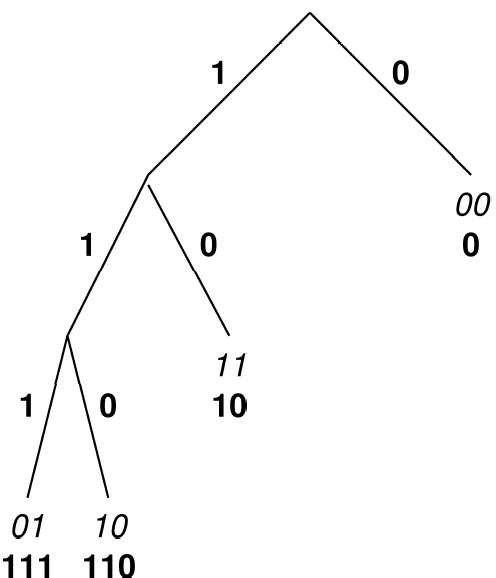
\includegraphics[scale=0.1]{figure1.png}%
 		\caption{Tree}\label{fig:baum}%
 	\end{center}%
\end{figure}

\begin{table}[h]%
 	\begin{center}%
		\caption{Some table}\label{tab:example}%
	 	\begin{tabular}{c|c}%
 			Column1 & Column2\\
 			\hline
 			0 & 1\\
 		\end{tabular}%
 	\end{center}%
\end{table}


\section{Case Studies}\label{sec:case-studies}

\subsection{Google and YouTube's Data Collection on Children}\label{subsec:google-and-youtube's-data-collection-on-children}
In 2019, Google and YouTube were fined \$170 million by the FTC for violating the Children’s Online Privacy Protection Act (COPPA). They had collected personal information from children under 13 without parental consent, raising significant privacy concerns and violating ethical principles of informed consent.
This case highlights the vulnerability of children in the digital age and the need for stricter regulations to protect their privacy.

The ethical implications of this case are profound.
Children, as a vulnerable population, require special protections.
Collecting data without parental consent not only violates legal standards but also ethical norms of safeguarding minors.
The lack of transparency and informed consent in this case undermines trust in digital platforms and calls for more robust regulatory frameworks to ensure ethical data practices.

\subsection{Google+ Data Breach}\label{subsec:google+-data-breach}
In 2018, Google announced that a software glitch in Google+ had exposed private data of up to 500,000 users.
The breach, discovered in March 2018, was not disclosed immediately, raising issues of transparency and accountability.
The delayed disclosure prevented users from taking timely actions to protect their data, leading to potential harm and distrust.

The Google+ data breach underscores the importance of timely disclosure in maintaining trust and accountability.
From an ethical standpoint, withholding information about data breaches violates the principle of transparency and the duty to protect users' privacy.
The incident also highlights the need for better security measures and proactive communication strategies to manage data breaches effectively.

\subsection{Project Nightingale}\label{subsec:project-nightingale}
In 2019, it was revealed that Google had partnered with Ascension to collect and analyze health data of millions of Americans without informing them.
This project raised significant privacy concerns and issues related to informed consent.
The use of sensitive health data without explicit consent undermines trust in healthcare providers and digital services.

The ethical concerns surrounding Project Nightingale revolve around the unauthorized use of sensitive health information.
Health data is inherently personal and requires stringent protections.
The lack of informed consent and transparency in this case breaches ethical standards and poses risks to patient privacy and autonomy.
This case illustrates the need for ethical guidelines and regulations in handling health data.

\subsection{Google’s Location Tracking}\label{subsec:googles-location-tracking}
In 2018, an investigation by the Associated Press found that Google continued to track users' location even when they had turned off location tracking settings, which was seen as deceptive and a violation of privacy.
This practice highlights the discrepancy between user expectations and actual data practices, leading to ethical concerns about honesty and transparency.

Google's location tracking practices raise ethical questions about deception and respect for user preferences.
Despite user actions to disable location tracking, continued data collection violates privacy and autonomy.
This case emphasizes the importance of aligning data practices with user expectations and ensuring that privacy controls are effective and respected.

\subsection{Google Street View Wi-Fi Data Collection}\label{subsec:google-street-view-wi-fi-data-collection}
Between 2007 and 2010, Google Street View cars inadvertently collected data from unencrypted Wi-Fi networks, including personal emails and passwords.
This incident highlighted unauthorized data collection and lack of transparency.
The inadvertent nature of the data collection does not absolve Google of responsibility, as it indicates inadequate safeguards and oversight.

The ethical issues in this case involve unauthorized data collection and the lack of transparency in Google's actions.
Collecting personal data without consent breaches privacy and trust.
The incident underscores the need for robust data governance practices and transparent communication with users about data collection activities.

\subsection{Incognito Mode Tracking Lawsuit}\label{subsec:incognito-mode-tracking-lawsuit}
In 2020, a class-action lawsuit was filed against Google for allegedly continuing to track users' internet activity even in Incognito mode, designed for private browsing.
This raised significant ethical concerns about privacy and deception.
The promise of privacy in Incognito mode is contradicted by the continued tracking, undermining user trust and autonomy.

The ethical implications of tracking users in Incognito mode are significant.
Promising privacy and then violating it not only undermines user trust but also breaches the ethical principles of honesty and respect for user autonomy.
Users rely on Incognito mode for private browsing, and violating this expectation of privacy is a serious ethical breach.

\section{Ethical Frameworks}\label{sec:ethical-frameworks}

\subsection{Deontological Perspective}\label{subsec:deontological-perspective}
Google's data practices often violate principles of autonomy and consent.
Users are typically not fully informed about the extent of data collection, which infringes on their autonomy and right to privacy.
According to Kantian ethics, this is inherently unethical as it fails to respect the intrinsic worth of individuals, violating the principle of treating people as ends in themselves.
Additionally, Kant's principle of the categorical imperative suggests that actions are only morally right if they can be universalized.
The practice of collecting personal data without consent cannot be ethically justified as a universal law because it would lead to a society where privacy is routinely violated, undermining trust and freedom.
\subsection{Contractualist Perspective}\label{subsec:contractualist-perspective}
The implicit agreement between Google and its users is often unfair, with users not adequately informed about how their data will be used.
This lack of transparency undermines trust and the social contract.
Contractualists would argue that data practices should be based on fair agreements that all parties, including users, would consent to under reasonable conditions.
Furthermore, the principle of reciprocity is violated as users provide valuable data without receiving fair compensation or benefits in return.
The imbalance of power and information between Google and its users creates an unethical dynamic where users are exploited for their data.
\subsection{Consequentialist Perspective}\label{subsec:consequentialist-perspective}
Google's services provide significant benefits, including enhanced user experience and economic growth.
However, these benefits are countered by privacy invasions, potential for data breaches, and manipulation of user behavior.
From a utilitarian perspective, the overall consequences of surveillance capitalism might not justify the means if the negative impacts on individual and societal well-being are substantial.
The long-term consequences of widespread data collection include the erosion of trust in digital services, increased anxiety and mental health issues related to privacy concerns, and potential misuse of data by malicious actors.
These negative outcomes must be weighed against the economic and convenience benefits provided by personalized services.
\subsection{Hedonistic Perspective}\label{subsec:hedonistic-perspective}
While Google's services increase user pleasure through convenience and personalization, the anxiety and distress caused by privacy concerns and data misuse result in significant net pain.
A hedonist would weigh the pleasure and pain resulting from surveillance capitalism to determine its ethicality.
If the negative impacts on well-being are substantial, the practice might be deemed unethical.
The subjective nature of pleasure and pain also highlights the diversity of user experiences.
While some users may greatly benefit from personalized services, others may suffer from the constant surveillance and lack of privacy, leading to a more complex ethical evaluation.

%\input{section2}


\section{Conclusion}
\noindent blabla


%%%%%%%%%%%%%%%%%%%%%%%%%%%%%%%%%%%%%%%%%%%%%%%%%%%%%%%%%%%%%%%%%%%%%%%%%%
% 	Acknowledgements
%%%%%%%%%%%%%%%%%%%%%%%%%%%%%%%%%%%%%%%%%%%%%%%%%%%%%%%%%%%%%%%%%%%%%%%%%%

%\section*{Acknowledgment}
%\addcontentsline{toc}{section}{Acknowledgment}

%%%%%%%%%%%%%%%%%%%%%%%%%%%%%%%%%%%%%%%%%%%%%%%%%%%%%%%%%%%%%%%%%%%%%%%%%%
% 	References
%%%%%%%%%%%%%%%%%%%%%%%%%%%%%%%%%%%%%%%%%%%%%%%%%%%%%%%%%%%%%%%%%%%%%%%%%%

% trigger a \newpage just before the given reference
% number - used to balance the columns on the last page
% adjust value as needed - may need to be readjusted if
% the document is modified later
%\IEEEtriggeratref{8}
% The "triggered" command can be changed if desired:
%\IEEEtriggercmd{\enlargethispage{-5in}}

% references section
% NOTE: BibTeX documentation can be easily obtained at:
% http://www.ctan.org/tex-archive/biblio/bibtex/contrib/doc/

% can use a bibliography generated by BibTeX as a .bbl file
% standard IEEE bibliography style from:
% http://www.ctan.org/tex-archive/macros/latex/contrib/supported/IEEEtran/bibtex
\bibliographystyle{IEEEtran}
% argument is your BibTeX string definitions and bibliography database(s)
\bibliography{IEEEabrv,references}
%
% <OR> manually copy in the resultant .bbl file
% set second argument of \begin to the number of references
% (used to reserve space for the reference number labels box)
%\begin{thebibliography}{1}
%
%\bibitem{ref:kopka}
%H.~Kopka and P.~W. Daly, \emph{A Guide to {\LaTeX}}, 3rd~ed.\hskip 1em plus
%  0.5em minus 0.4em\relax Harlow, England: Addison-Wesley, 1999.
%
%\end{thebibliography}

%%%%%%%%%%%%%%%%%%%%%%%%%%%%%%%%%%%%%%%%%%%%%%%%%%%%%%%%%%%%%%%%%%%%%%%%%%
% 	End of the document
%%%%%%%%%%%%%%%%%%%%%%%%%%%%%%%%%%%%%%%%%%%%%%%%%%%%%%%%%%%%%%%%%%%%%%%%%%

\end{document}


